\documentclass[]{article}
\usepackage{booktabs, adjustbox} % Tables
\usepackage{graphicx} % Images graphics
\usepackage{float}    % For floats
\usepackage{siunitx}  % For SI Units
\usepackage{amsmath}  % For multiple math equations
\graphicspath{{../img/}}



\title{ENPHYS253 \\ Lab 5: Bending Beams and Strain Gauges}
\author{Viraj Bangari \\ 10186046}
\date{\today}

\newcommand{\gaugeOneTheoretical}{\ensuremath{(1.32 \pm 0.01) * 10^{-4}
\si{\per\meter}}}
\newcommand{\gaugeTwoTheoretical}{\ensuremath{(8.78 \pm 0.03) * 10^{-5} \si{\per\meter}}}
\newcommand{\gaugeThreeTheoretical}{\ensuremath{(4.55 \pm 0.01) * 10^{-5} \si{\per\meter}}}

\newcommand{\gaugeOneMeasured}{\ensuremath{(1.21 \pm 0.01) * 10^{-4} \si{\per\meter}}}
\newcommand{\gaugeTwoMeasured}{\ensuremath{(8.10 \pm 0.02) * 10^{-5} \si{\per\meter}}}
\newcommand{\gaugeThreeMeasured}{\ensuremath{(4.12 \pm 0.07) * 10^{-5} \si{\per\meter}}}

\newcommand{\weightSlope}{\ensuremath{(2.19 \pm 0.02) * 10^{-4} \si{\per\newton}}}
\newcommand{\youngsMeasured}{\ensuremath{70 \pm 1 \si{\giga\pascal}}}
\newcommand{\youngsTheoretical}{\ensuremath{69 \si{\giga\pascal}}}

\newcommand{\compressionSlope}{\ensuremath{(1.14 \pm 0.01) * 10^{-4}
\si{\per\newton}}}

\newcommand{\ratio}{\ensuremath{-0.322 \pm 0.002}}
\newcommand{\poissonMeasured}{\ensuremath{0.322 \pm 0.002} \si{\giga\pascal}}
\newcommand{\poissonTheoretical}{\ensuremath{0.32} \si{\giga\pascal}}

%% Measurements of beam
\newcommand{\xOne}{\ensuremath{25.5 \pm 0.01 \si{\milli\meter}}}
\newcommand{\xTwo}{\ensuremath{101.66 \pm 0.01 \si{\milli\meter}}}
\newcommand{\xThree}{\ensuremath{175.5 \pm 0.01 \si{\milli\meter}}}

\newcommand{\xTop}{\ensuremath{25 \pm 0.5 \si{\milli\meter}}}
\newcommand{\xBottom}{\ensuremath{26 \pm 0.5 \si{\milli\meter}}}

\newcommand{\GF}{\ensuremath{2.0}}
\newcommand{\Kt}{\ensuremath{0.01}}

\newcommand{\LOne}{\ensuremath{255 \pm 0.5 \si{\milli\meter}}}
\newcommand{\LTwo}{\ensuremath{286 \pm 0.5 \si{\milli\meter}}}
\newcommand{\LThree}{\ensuremath{252 \pm 0.5 \si{\milli\meter}}}

\newcommand{\aOne}{\ensuremath{6.33 \pm 0.01 \si{\milli\meter}}}
\newcommand{\bOne}{\ensuremath{25.61 \pm 0.01 \si{\milli\meter}}}

\newcommand{\aTwo}{\ensuremath{6.0 \pm 0.5 \si{\milli\meter}}}
\newcommand{\bTwo}{\ensuremath{26.0 \pm 0.5 \si{\milli\meter}}}

\begin{document} 
\maketitle

\section{Theory}
A cantilever beam that is fixed on one end and with forced displacement on the
other has its longitudinal strain $\epsilon_l$ determined by this equation:
\begin{equation}
    \epsilon_l = \frac{3a(L-x)}{2L^3}y \tag{\ref{eq:longitudinal}}
\end{equation}
where $x$ is the distance between the fixed point and the point of strain, $a$
is thickness of beam and $L$ is the distance between the
fixed point and the applied force. If the force is known, the strain can be found by
using:
\begin{equation}
    \epsilon_l = \frac{6(L-x)}{a^2bY}W \tag{\ref{eq:force}}
\end{equation}
where $Y$ is the Young's modulus of the material, $b$ is width of beam, and $W$
is the applied force.  If the beam is subject to uniaxial stress, it exhibits
transversal strain $\epsilon_t$. The Poisson's ratio, $\sigma$ of the material
can be found as the negative ratio between transverse and longitudinal stress:
\begin{equation}
    \sigma = -\frac{\epsilon_t}{\epsilon_l} \tag{\ref{eq:poisson}}
\end{equation}

For physically measuring the value of strain, a strain gauge is used. They
typically consist of a layer of metal or semiconductor on a thin insulating film
and are bonded directly to the beam. As the beam bends, the resistance changes
as function of the strain. The calibration of the gauge called the gauge factor,
defined as $GF = \delta R/R/\epsilon_l$, where $\delta R/R$ is the relative
change in the resistance caused by the strain $\epsilon_l$. A gauge is designed
to be more sensitive when stretched in one direction than its perpendicular, and
ratio of the two sensitivities is called the transverse sensitivity $K_t$. This
means that for a transverse strain, the measured value contains a significant
error. To correct for the error the following equation is used:
\begin{equation}
    \epsilon_t = \epsilon_t^{'} - K_t\epsilon_l \tag{\ref{eq:transverse}}
\end{equation}
where $\epsilon_t^{'}$ is the strain measured by the gauge.

\section{Results and Analysis}
The longitudinal strains caused by the micrometer for the three gauges in
table~\ref{tab:strain1} were plotted onto
figures~\ref{fig:gauge1},~\ref{fig:gauge2} and~\ref{fig:gauge3}. A linear
regression was performed, resulting in slopes of \gaugeOneTheoretical,
\gaugeTwoTheoretical, \gaugeThreeTheoretical\ for gauge 1, gauge 2 and gauge 3
respectively. The theoretical values for these slopes were calculated using
equation~\ref{eq:transverse} and were determined as \gaugeOneMeasured,
\gaugeTwoMeasured\ and \gaugeThreeMeasured. None of these values overlap,
indicating a systematic error.

The longitudinal strains in gauge 1 caused by varying masses were recorded in
table~\ref{tab:strain2} and were plotted onto figure~\ref{fig:weight}. A
linear regression was performed, resulting in a slope of \weightSlope. This
value was used with equation~\ref{eq:young} (found in the appendix), determining the
Young's modulus of the aluminum beam as \youngsMeasured. This value agrees with
the theoretical value of \youngsTheoretical for aluminum~\cite{ref:young}.

The compression strains in gauge 1 caused by the micrometer were
recorded in table~\ref{tab:strain3} and were plotted on
figure~\ref{fig:compression}. After a linear regression was performed, the slope
was determined as \compressionSlope. Though this value of the slope was expected
to be equal in magnitude to the slope of figure~\ref{fig:gauge1}, the values do
not overlap.

Using a different beam, the longitudinal and transverse strains on their
respective gauges were measured onto table~\ref{tab:strain4}. The transverse
strain data was corrected using equation~\ref{eq:transverse} and was plotted on
figure~\ref{fig:transverse}. The longitudinal strain data was plotted on
figure~\ref{fig:longitudinal}. The transverse and longitudinal data points were
plotted against each other on figure~\ref{fig:poisson}, and a linear regression
determined the ratio between the two strains as \ratio.
Equation~\ref{eq:poisson} was used with this value to determine that the
Poisson's ratio of the aluminum beam was \poissonMeasured, agreeing with the
accepted value of \poissonTheoretical~\cite{ref:poisson}.


\newpage
% Part 1
\begin{figure}[hp]
    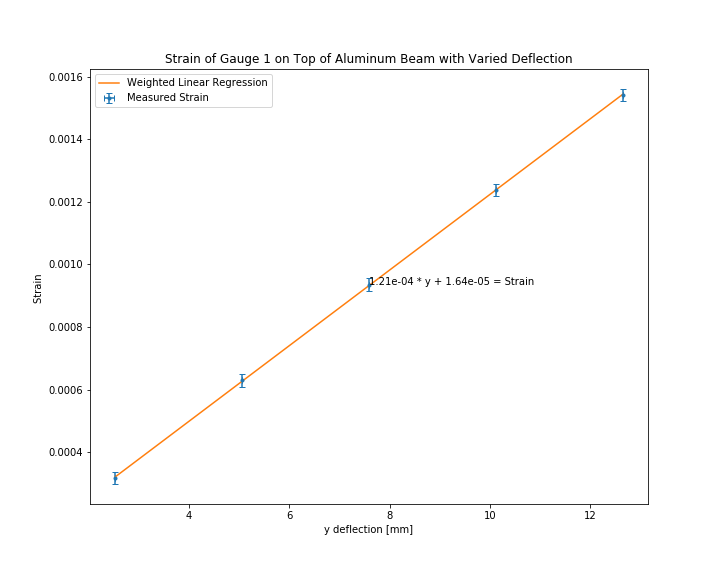
\includegraphics[width=\textwidth]{../output/graph/gauge1Strain.png}
    \caption{Strain of Gauge 1 on Top of Aluminum Beam with Varied Deflection
    with $L=$ \LOne, $x=$ \xOne\ and $GF=$ \GF}\label{fig:gauge1}
\end{figure}

\newpage
\begin{figure}[hp]
    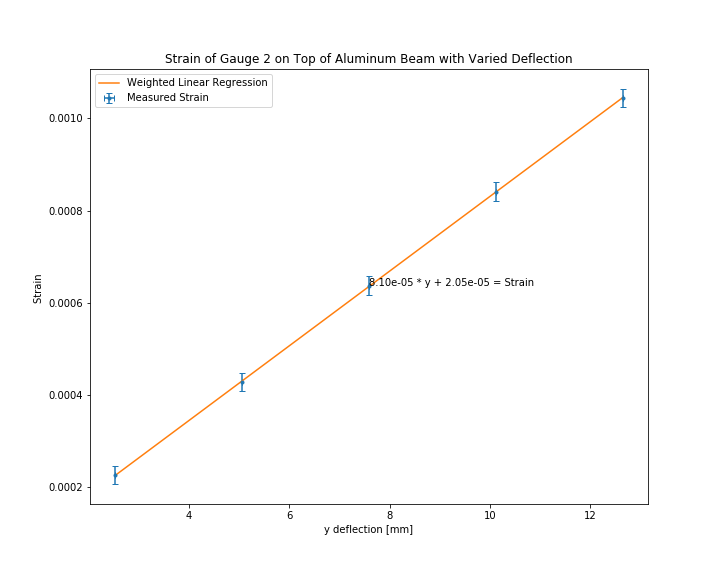
\includegraphics[width=\textwidth]{../output/graph/gauge2Strain.png}
    \caption{Strain of Gauge 2 on Top of Aluminum Beam with Varied Deflection
    with $L=$ \LOne, $x=$ \xTwo\ and $GF=$ \GF}\label{fig:gauge2}
\end{figure}

\newpage
\begin{figure}[hp]
    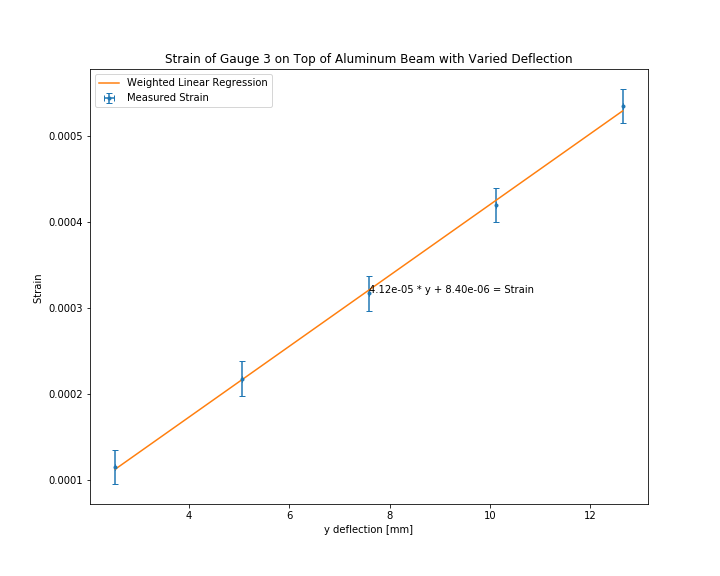
\includegraphics[width=\textwidth]{../output/graph/gauge3Strain.png}
    \caption{Strain of Gauge 3 on Top of Aluminum Beam with Varied Deflection
    with $L=$ \LOne, $x=$ \xThree\ and $GF=$ \GF}\label{fig:gauge3}
\end{figure}

% Part 2
\newpage
\begin{figure}[hp]
    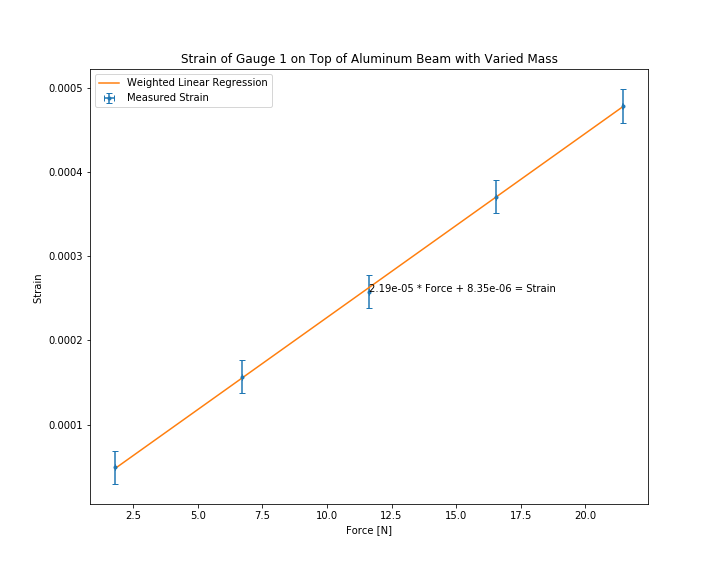
\includegraphics[width=\textwidth]{../output/graph/weightStrain.png}
    \caption{Strain of Gauge 1 on Top of Aluminum Beam with Varied
    Mass with $L=$ \LTwo, $x=$ \xOne\ and $GF=$ \GF}\label{fig:weight}
\end{figure}

% Part 3
\newpage
\begin{figure}[hp]
    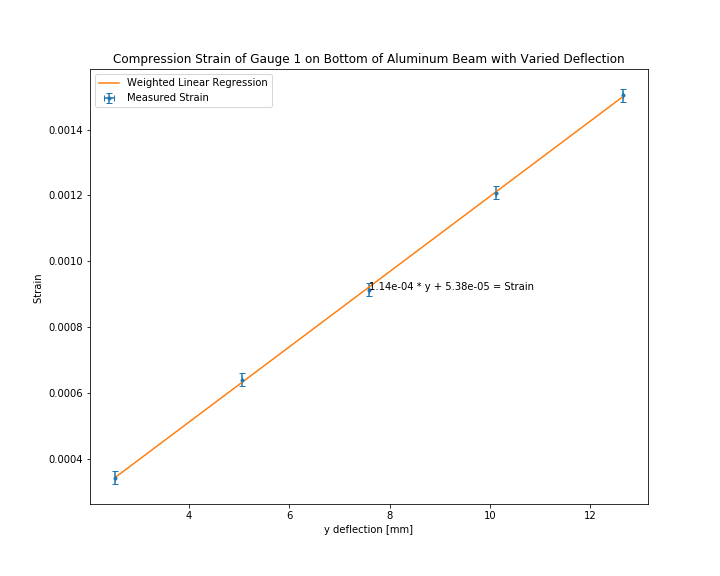
\includegraphics[width=\textwidth]{../output/graph/compressionStrain.png}
    \caption{Compression Strain of Gauge 1 on Bottom of Aluminum Beam with
    Varied Deflection with $L=$ \LTwo, $x=$ \xOne\ and $GF=$ \GF}\label{fig:compression}
\end{figure}

% Part 4
\newpage
\begin{figure}[hp]
    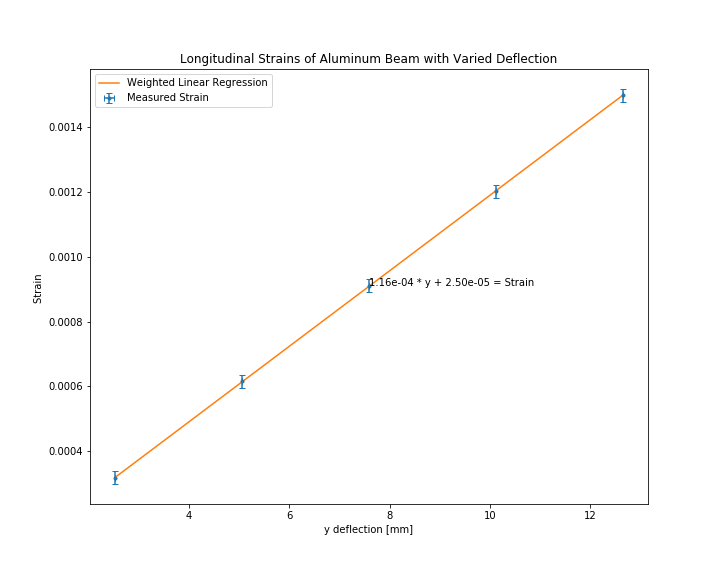
\includegraphics[width=\textwidth]{../output/graph/longitudinal.png}
    \caption{Longitudinal Strain of Gauge 1 on Bottom of Aluminum Beam with
    Varied Deflection with $L=$ \LThree, $x=$ \xTop\ and $GF=$ \GF}\label{fig:longitudinal}
\end{figure}

\newpage
\begin{figure}[hp]
    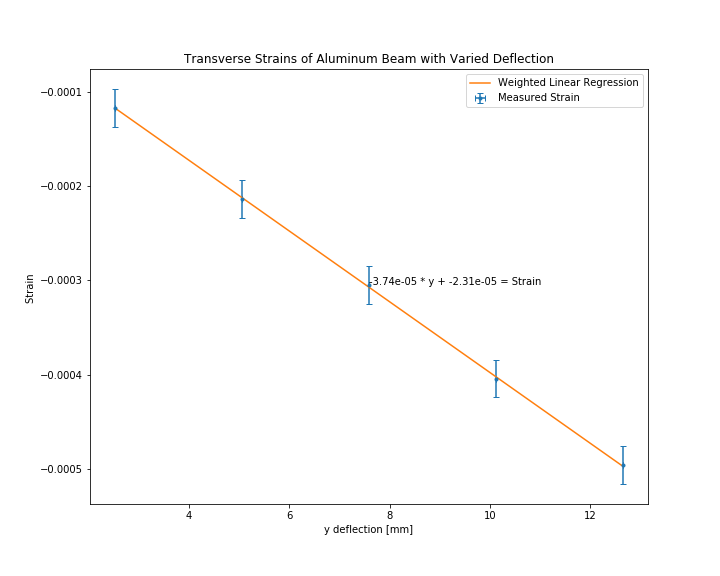
\includegraphics[width=\textwidth]{../output/graph/transverse.png}
    \caption{Transverse Strain of Gauge 1 on Bottom of Aluminum Beam with
    Varied Deflection with $L=$ \LThree, $x=$ \xBottom\ and $GF=$ \GF}\label{fig:transverse}
\end{figure}

\newpage
\begin{figure}[hp]
    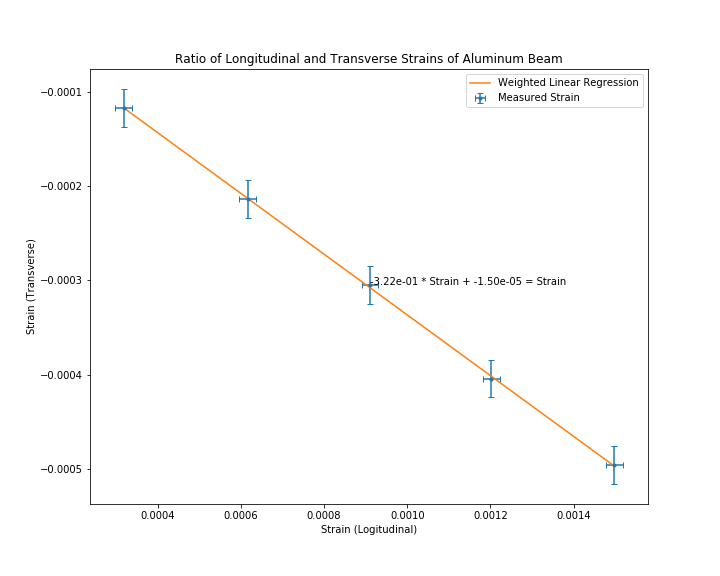
\includegraphics[width=\textwidth]{../output/graph/poisson.png}
    \caption{Ratio of Longitudinal and Transverse Strains of Aluminum
    Beam with $L=$ \LThree\ and $GF=$ \GF}\label{fig:poisson}
\end{figure}

\newpage
\section{Appendix}
\subsection{Equation List} 

\begin{equation}\label{eq:longitudinal}
    \epsilon_l = \frac{3a(L-x)}{2L^3}y
\end{equation}
$\epsilon_l$ is longitudinal strain, $a$ is thickness of beam, $b$ is width
of beam, $x$ is the distance between the clamp and the gauge, $y$ is the
deflection length and $L$ is the distance between the clamp and the force.

\begin{equation}\label{eq:force}
    \epsilon_l = \frac{6(L-x)}{a^2bY}W
\end{equation}
$Y$ is Young's modulus, $W$ is the force at the end of the beam.


\begin{equation}\label{eq:poisson}
    \sigma = -\frac{\epsilon_t}{\epsilon_l}
\end{equation}
$\sigma$ is Poisson's ratio, $\epsilon_t$ is the transverse strain.

\begin{equation}\label{eq:transverse}
    \epsilon_t = \epsilon_t^{'} - K_t\epsilon_l
\end{equation}
$\epsilon_t$ is the corrected transverse strain, $\epsilon_t^{'}$ is the measured
transverse strain and $K_t$ is the transverse sensitivity.

\begin{equation}\label{eq:young}
    Y = \frac{1}{\frac{a^2 * b}{6(L-x)}\frac{\epsilon_l}{W}}
\end{equation}
Note: this is equation~\ref{eq:force} rearranged for $Y$.

\subsection{Raw Data}

\begin{table}[H]
    \caption{Strain Measurements for Aluminum Beam using Micrometer with with
    $L=$ \LOne, $x_1=$ \xOne\, $x_2=$ \xTwo\, $x_3=$ \xThree, $GF= $ \GF, $a= $
    \aOne, $b= $\bOne, and $K_t=$ \Kt.
    }\label{tab:strain1}
    \begin{tabular}{@{}p{2cm}p{3cm}p{3cm}p{3cm}@{}}
        \toprule
        Deflection [in] & Gauge 1 Strain *  10\textasciicircum -5 +/- 2 * 10\textasciicircum -5 & Gauge 2 Strain *  10\textasciicircum -5 +/- 2 * 10\textasciicircum -5 & Gauge 3 Strain * 10\textasciicircum -5 +/- 2 * 10\textasciicircum -5 \\ \midrule
        0.1                 & 31.8                                                                  & 22.6                                                                  & 11.5                                                                 \\
        0.2                 & 63                                                                    & 42.8                                                                  & 21.8                                                                 \\
        0.3                 & 93.6                                                                  & 63.7                                                                  & 31.7                                                                 \\
        0.4                 & 123.8                                                                 & 84.1                                                                  & 42                                                                   \\
        0.5                 & 154.1                                                                 & 104.4                                                                 & 53.5                                                                 \\ \bottomrule
    \end{tabular}
\end{table}

\begin{table}[H]
    \caption{Strain Measurements for Aluminum Beam using Mass with with
    $L=$ \LTwo, $x=$ \xOne, $GF= $ \GF, $a= $ \aOne, $b= $\bOne, and $K_t=$ \Kt.
    }\label{tab:strain2}
    \begin{tabular}{@{}lll@{}}
        \toprule
        Mass [g] & Error in Mass [g] & Gauge Strain  * 10\textasciicircum -5 +/- 2 * 10\textasciicircum -5 \\ \midrule
        184.87       & 0.2                   & 4.9                                                                 \\
        685.58       & 0.4                   & 15.7                                                                \\
        1186.43      & 0.4                   & 25.8                                                                \\
        1687.14      & 0.6                   & 37.1                                                                \\
        2187.84      & 0.4                   & 47.9                                                                \\ \bottomrule
    \end{tabular}
\end{table}

\begin{table}[H]
    \caption{Compression Strain Measurements for Aluminum Beam using Mass with with
    $L=$ \LOne, $x=$ \xOne, $GF= $ \GF, $a= $ \aOne, $b= $\bOne, and $K_t=$ \Kt.
    }\label{tab:strain3}
    \begin{tabular}{@{}ll@{}}
        \toprule
        Deflection [in] & Strain *  10\textasciicircum -5 +/- 2 * 10\textasciicircum -5 \\ \midrule
        0.1                 & 34.2                                                          \\
        0.2                 & 64                                                            \\
        0.3                 & 91.3                                                          \\
        0k.4                 & 120.8                                                         \\
        0.5                 & 150.4                                                         \\ \bottomrule
    \end{tabular}
\end{table}

\begin{table}[H]
    \caption{Compression Strain Measurements for Aluminum Beam using Mass with with
    $L=$ \LTwo, $x_{longitudinal}=$ \xTop, $x_{transverse} =$ \xBottom, $GF= $
    \GF, $a= $ \aTwo, $b= $\bTwo, and $K_t=$ \Kt.
    }\label{tab:strain4}
    \begin{tabular}{@{}lp{4.5cm}p{4.5cm}@{}}
        \toprule
        Deflection [in] & Longitudinal Strain*  10\textasciicircum -5 +/- 2 * 10\textasciicircum -5 & Transverse Strain *  10\textasciicircum -5 +/- 2 * 10\textasciicircum -5 \\ \midrule
        0.1                 & 31.8                                                                      & 11.4                                                                      \\
        0.2                 & 61.6                                                                      & 20.8                                                                      \\
        0.3                 & 91                                                                        & 29.6                                                                      \\
        0.4                 & 120.2                                                                     & 39.2                                                                      \\
        0.5                 & 149.8                                                                     & 48.1                                                                      \\ \bottomrule
    \end{tabular}
\end{table}

\subsection{Sample Calculations}
\subsubsection{Theoretical Slope for Gauge 1}
$= \frac{3a(L-x)}{2L^3} $

$= \frac{3 * \aOne (\LOne - \xOne)}{2 * {(\LOne)}^3}$

$= \gaugeOneTheoretical$

\subsubsection{Theoretical Slope for Gauge 2}

$= \frac{3a(L-x)}{2L^3}$

$= \frac{3 * \aOne (\LOne - \xTwo)}{2 * {(\LOne)}^3}$

$ = \gaugeTwoTheoretical$

\subsubsection{Theoretical Slope for Gauge 3}

$= \frac{3a(L-x)}{2L^3}$ 

$= \frac{3 * \aOne (\LOne - \xThree)}{2 * {(\LOne)}^3}$

$ = \gaugeThreeTheoretical$

\subsubsection{Young's Modulus}

$= \frac{1}{\frac{{(\aOne)}^2 * \bOne}{6(\LOne-\xOne)} * \weightSlope}$

$= \youngsMeasured$

\subsubsection{Poisson's Ratio}

$= -\frac{\epsilon_t}{\epsilon_l} $

$= -\weightSlope $

$= \poissonMeasured$

\bibliographystyle{ieeetr}%Used BibTeX style is unsrt
\bibliography{lab5}
\end{document}
